\chapter{Design and Implementation}

Use \url{https://docs.google.com/document/d/1tCYCOFDeL8E3USIOunRNrqh6ekP_-kAQVHMrNJ4jk04} and the source code to complete. This section will probably need extensive, in-depth discussion of the algorithms we use, supported by diagrams for each part...

Should include discussion of technical challenges...

\section{Background}

\subsection{Architectural overview}

Diagram...

A full example query...

These are the components and their interactions...

Before vs after...

\subsection{Voodoo vector algebra}

This is what Voodoo is, how it works, and what it does (use \url{http://www.vldb.org/pvldb/vol9/p1707-pirk.pdf})...

Talk about existing architecture using monetdb and printer/planeater...

\subsection{Apache Calcite}

\emph{Apache Calcite} \cite{Begoli:2018:ACF:3183713.3190662} is a software framework that provides query language support, query optimisation and query processing, and is used by several popular data processing systems.

Whilst Calcite is written entirely in Java, which makes interaction with the Voodoo kernel difficult, Calcite was chosen as the framework on which to develop our front-end, thanks to its fairly widespread adoption, open-source friendliness and stability. By building on top of Calcite, we benefit from not having to entirely implement SQL parsing and validation, JDBC compliancy, and default operator implementations (which are useful when the Voodoo implementation of an operator would be beyond the scope of this project) ourselves.

\subsubsection{Architecture of Apache Calcite}

\begin{figure}
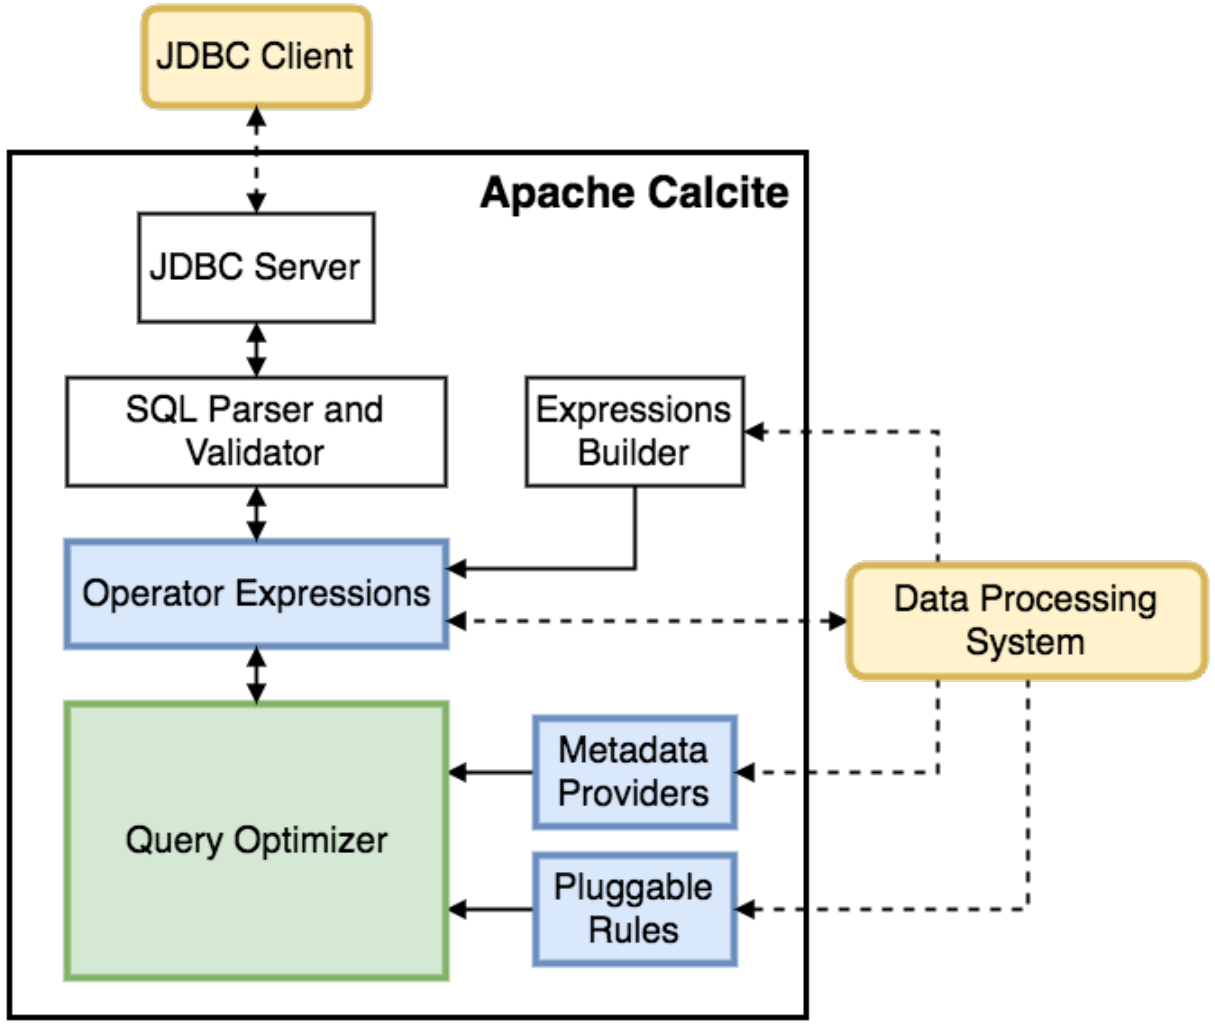
\includegraphics[width=0.5\textwidth]{design-and-implementation/calcite-architecture.png}
\centering
\caption{Architecture of Apache Calcite \cite{Begoli:2018:ACF:3183713.3190662}}
\label{fig:calcite-architecture}
\end{figure}

Calcite consists of most of the components needed to make a DBMS, with three significant omissions: algorithms to process data, storage of data, and a catalog for metadata. Figure \ref{fig:calcite-architecture} shows an overview of its architecture and interactions.

Firstly, Calcite provides a JDBC server (\emph{Avatica}), as well as a default implementation of its SPI. Alternatively, an application can use Avatica's JDBC driver directly (which is the approach we take with our web-interface).

Calcite then supports query evaluation in each of the following stages:
\begin{enumerate}
    \item \textbf{Parsing} the SQL query. Calcite provides an LL($k$) parser generated by JavaCC, and developers usually need not consider this step beyond setting some basic configuration options.
    \item \textbf{Validating} the SQL query. Calcite validates queries against any known metadata. Developers need to provide an interface that allows Calcite to get this metadata for a table (an \emph{adapter}).
    \item \textbf{Optimising} the logical plan, and converting it to physical expressions. Calcite can do this with some help. It provides two algorithms for rule-based logical query optimisation, as well as around one-hundred rules. However, developers will likely need to add further rules, including rules to rewrite a logical plan into physical expressions for their application.
    \item \textbf{Executing} the physical plan, by converting it into application-specific executions. Calcite can handle this in simple cases, say where the application actually supports SQL input (i.e. Calcite is just being used as an optimiser). In other cases, such as ours, this step requires a lot of application-specific code to be written.
\end{enumerate}

\subsubsection{Relational algebra}

Calcite uses relational algebra \cite{Codd:1970:RMD:362384.362685} to express queries. Specifically, it builds a tree of \texttt{RelNode}s, each of which represent a relational operator. Each \texttt{RelNode} could represent, for example, a \texttt{TableScan}, \texttt{Project}, \texttt{Filter}, \texttt{Aggregate}, \texttt{Join}, \texttt{Union}, \texttt{Intersect} or \texttt{Sort}.

Projection and sort fields, as well as filter and join conditions, are expressed by trees of \texttt{RexNode}s. A \texttt{RexNode} represents a row-level expression, and its implementations include \texttt{RexCall} (an operation such as "add" or "is equal to"), \texttt{RexInputRef} (a reference to an input column) and \texttt{RexLiteral} (a literal value), as well as many others (which we do not consider).

Relational expressions are associated with \emph{traits} (\texttt{RelTrait}s), which describe their physical properties, such as ordering, grouping, or partitioning. The most important trait, however, is the \emph{calling convention} (\texttt{Convention}), which specifies the data processing system where the expression will be executed. The \texttt{Logical} calling convention is used when no implementation has been selected.

\subsubsection{Query processing and optimisation}

Calcite includes \emph{planner rules} (\texttt{RelOptRule}s) to transform expression trees. Each rule defines a condition on the original tree, and a conversion, that rewrites part of the tree. Calcite provides common rules, such as the \texttt{FilterIntoJoinRule}, which pushes a filter into a join where possible, to reduce the work in the join. Developers also must provide their own rules to transform the tree from a logical to an optimised physical plan.

Calcite also provides two planner engines (\texttt{RelOptPlanner}s) to apply these rules: one requires a cost-model and uses a dynamic programming algorithm, similar to Volcano's \cite{Graefe:1994:VEP:627290.627558} (\texttt{VolcanoPlanner}), whilst the other exhaustively applies rules until it reaches a fixpoint (\texttt{HepPlanner}).

\subsubsection{Adapters}

As Calcite does not include a storage layer, it requires developers to build an \emph{adapter}. Figure \ref{fig:calcite-adapter} shows the design of a minimal adapter:
\begin{itemize}
    \item The \texttt{Model} is a JSON-formatted description of the physical properties of the data source being accessed.
    \item The \texttt{Schema} is a definition of the data found in the model, and is generated by a \texttt{SchemaFactory} for the adapter. Usually this will use a \texttt{TableFactory}, which generates a \texttt{Table} defining the names and types of the columns in each table, as well as any statistics available, such as cardinalities, distributions, and which columns are keys.
\end{itemize}

An adapter also usually provides a set of rules to be added to the planner. Specifically, rules to rewrite logical operators to physical operators of the adapter's convention.

The minimal rule set includes a translation for table-scans, which implement the access paths for tables in the adapter. Once Calcite can read the data, it can implement all other operators using the \texttt{Enumerable} calling convention, which uses a conventional iterator implementation written in Java.

Rules are also used to convert all other operators, to avoid plans relying too heavily on costly \texttt{Enumerable} operators. Each of these rules, in our case, defines an implementation instead using the \texttt{Voodoo} convention.

\begin{figure}
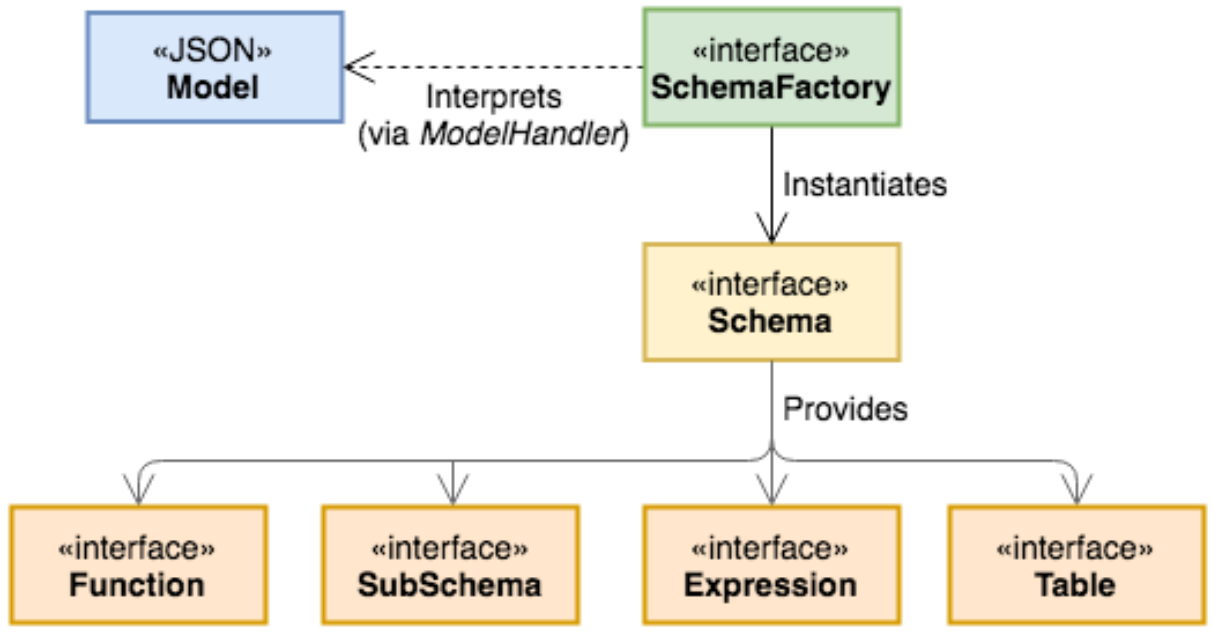
\includegraphics[width=0.5\textwidth]{design-and-implementation/calcite-adapter.png}
\centering
\caption{A minimal adapter for Apache Calcite \cite{Begoli:2018:ACF:3183713.3190662}}
\label{fig:calcite-adapter}
\end{figure}

\subsection{SWIG}

This is what SWIG is, how it works, and what it does (I guess \url{http://www.swig.org/Doc1.3/Java.html}?)...

\subsection{LibClang}

This is what LibClang is, how it works, and what it does (I guess \url{https://clang.llvm.org/doxygen/group__CINDEX.html}?)...

\subsection{OpenCL}

This is what OpenCL is, how it works, and what it does...

(CUDA?)

\section{Generating Voodoo from SQL using Apache Calcite}

Description of what Apache Calcite gives us...

\subsection{Defining schemas and importing data}

We don't have an explicit storage manager / catalog, so we use byte buffers...

We have a SchemaFactory which...

We have a TableFactory which then ... based on supported types...

\subsection{Translating logical operators to Voodoo}

Description of overall algorithm to convert logical plan -> voodoo (rules)...

For each logical operator, description of logical plan -> voodoo...

Using enumerables for other things...

\subsection{Translating row expressions to Voodoo}

Description of overall algorithm to convert row expression -> voodoo (visitor)...

For each row expression, description of expr -> voodoo...

\subsection{Communicating with the Voodoo Kernel}

Printer implementation...

Discussion of SWIG API...

How we pass values in for ClangAST implementation...

How we get values back for ClangAST implementation...

Technical challenges to do with garbage collection etc....

\subsection{Graphical web-interface}

We additionally provide a graphical front-end on top of our Calcite adapter, which displays the Calcite plan, Voodoo vector expressions, OpenCL and result for a query on the TPC-H schema.

\subsubsection{Purpose}

Building an interface was not an explicit goal of this project, and we do not expect it to be heavily used. However, the graphical web-interface's purpose is threefold:

\begin{enumerate}
\item It shows very clearly the transformations we make to generate OpenCL code from an SQL query, and provides graphical visualisations of the plan at various stages. As such, it is helpful for presenting the work we have done, and explaining how each intermediate representation is reached.
\item It provides a somewhat useful debugging interface. The alternative would be to use Apache Calcite's \texttt{sqlline} command-line interface. However, \texttt{sqlline} has several limitations. Firstly, there is a known issue whereby \texttt{sqlline} truncates long plans. Secondly, viewing the generated Voodoo vector expressions and the generated OpenCL require a different Voodoo implementations (\texttt{Printer} and \texttt{ClangAst} respectively), and hence different JDBC connections, which can be a little tedious to set up. The interface we have built does not require any such setup, and allows us to easily identify where a buggy query has gone wrong.
\item It proves that our database is JDBC-compliant, and provides sample Java code that includes connection configuration. It also shows how we can handle arbitrary SQL queries.
\end{enumerate}

\subsubsection{Implementation}

\begin{figure}
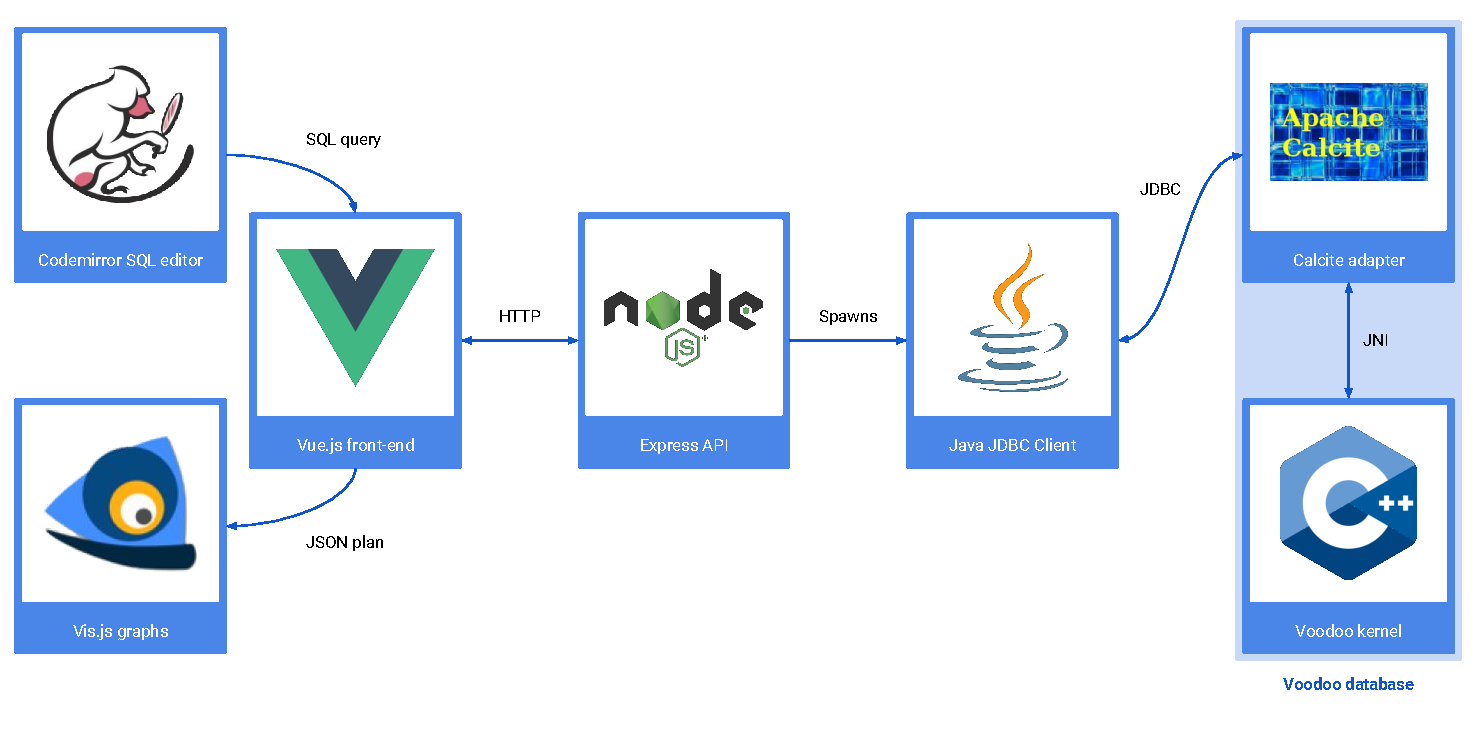
\includegraphics[width=\textwidth]{design-and-implementation/web-interface.pdf}
\centering
\caption{Architecture of the graphical web-interface}
\label{fig:web-interface}
\end{figure}

Figure \ref{fig:web-interface} shows the main components of the web-interface. Since this interface is not considered to be a real deliverable of this project, we favoured design decisions that allowed the most rapid development. As such we have:

\begin{enumerate}
\item A JDBC client, written in Java, that connects to our Voodoo implementation via the Calcite adapter. Note that the client never interacts directly with the Voodoo kernel, and so we rely on the kernel outputting Voodoo and OpenCL code, in addition to returning a result via the Calcite adapter. This approach provides a much cleaner interface than using an existing client, say \texttt{sqlline}, and avoids using unmaintained Node.js JDBC libraries.
\item An Express API, which accepts HTTP \texttt{GET} requests for a query. It returns a JSON, built from the output of the JDBC client, containing the plan, Voodoo, OpenCL and result for a query as well as any warnings or errors reported. This approach was much faster than using one of Java's more verbose HTTP server frameworks.
\item A Vue.JS frontend, which uses CodeMirror to provide an editor with SQL syntax highlighting and autocompletion. Queries are sent to the API, and we parse the response, using a hierarchical depth-first search starting from the returned vector, to build up the list of nodes and edges in a connected graph of the plan. The distances from the returned vector are used to define the $y$-coordinates ("levels") of operator nodes in the final graph, and vis.js then calculates $x$-coordinates using a physics simulation with spring forces between nodes.
\end{enumerate}

\section{Generating OpenCL from Voodoo using LibClang}

\subsection{Using LibClang to generate AST components}

We considered these options, and chose LibClang because...

For each component, description of how it is represented...

\subsection{Translating Voodoo to a Clang AST}

Description of overall algorithm to convert voodoo -> clang ast...

For each Voodoo API function, description of what it does and algorithm to convert it to AST...

\subsection{Generating and running OpenCL code}

Alternatives to OpenCL...

Generating fragments...

Running fragments...

Getting results...
